\documentclass[12pt]{article}



%\usepackage{refcheck}


\newcommand{\wss}[1]{\authornote{magenta}{SS}{#1}}
\newcommand{\ds}[1]{\authornote{blue}{DS}{#1}}

\usepackage{hyperref}
\usepackage{graphicx}
\graphicspath{ {Images/} }


\begin{document}

\title{Verification and Validation Plan for Solar Water Heating Systems Incorporating 
Phase Change Material} 
\author{Maya Grab}
\date{\today}
	
\maketitle

\tableofcontents

%%%%%%%%%%%%%%%%%%%%%%%%
%
%	1.) General Information 
%
%%%%%%%%%%%%%%%%%%%%%%%%

\section{General Information}
The following section provides an overview of the Test Plan 
for Smart Waiter Solutions.
 This section explains the purpose of this document, the scope of the system, and an overview of the following sections

%1.1 Purpose
\subsection{Purpose}
The purpose of this document is to describe the various test cases and procedures used  Smart Waiter.
This document is indented to be used as a reference for all future testing and will
be used to increase confidence in the software implementation.  

This document will be used as a starting point for the verification and validation report. The 
test cases presented within this document will be executed and the output will be analyzed to 
determine if the software is implemented correctly.  


%1.2 Scope
\subsection{Scope}



\subsection{Overview of Document }
The following sections provide more detail about the V\&V of a solar water heating
 simulator. Information about the testing process is provided, and the software specifications
that were discussed in the SRS document are stated.  The evaluation process that will be followed during 
testing is outlined, and test cases for both the system testing and unit testing are provided 

%%%%%%%%%%%%%%%%%%%%%%%%
%
%	2.) Plan
%
%%%%%%%%%%%%%%%%%%%%%%%%

\section{Plan}
This section provides a description of the software that is being tested, the team that will
perform the testing, the milestones for the testing phase, and the budget allocated to the testing. 

%2.1 Software Description
\subsection{Software Description}
The software being tested is a simulator for a SWHS
incorporating PCM. Given the physical parameters of the system,
 including dimensions, properties of the water and PCM,and relevant physical constants,
  the simulator calculates the changes in temperature and energy of the water and PCM 
  over time.

%2.2 Test Team
\subsection{Test Team} 
The team that will execute the test cases, write and review the V\&VR consists of:

\begin{itemize}
 \item Maya Grab 
 \item Dr.\ Spencer Smith
 \item Thulasi Jegatheesan 
\end{itemize}  

%2.3 Milestones
\subsection{Milestones}

%2.3.1 Location
\subsubsection{Location}
The location where the testing will be performed is Hamilton Ontario. The institution that
will be performing the testing is McMaster University. 


%2.3.1 Dates and Deadlines
\subsubsection{Dates and Deadlines}
%2.4 Budget
\subsection{Budget}
The budget for the testing of this system is being funded by McMaster University and NSERC.

%%%%%%%%%%%%%%%%%%%%%%%%
%
%	3.) Software Specification
%
%%%%%%%%%%%%%%%%%%%%%%%%

\section{ Software Specification}
This section provides the functional requirements, the business tasks that the
software is expected to complete, and the nonfunctional requirements, the
qualities that the software is expected to exhibit.

%3.1 Functional Requirements
\subsection{Functional Requirements}

\noindent
\begin{itemize}
\item Input the physical constants, properties and initial temperatures of water
 and PCM, and dimensions of the tank  
\item Verify that the inputs satisfy the required physical constraints 
\item Compute the calculated values required to solve the governing differential equations
\item Calculate the temperatures and energy of water and PCM over time.
\end{itemize} 

%3.2 Nonfunctional Requirements
\subsection{Nonfunctional Requirements}
Priority nonfunctional requirements are correctness, understandability,
reliability, and maintainability.


%%%%%%%%%%%%%%%%%%%%%%%%
%
%	4.) Test Types
%
%%%%%%%%%%%%%%%%%%%%%%%%

\section{Evaluation}
This section first presents the methods and constraints that are to be used
during the evaluation process. This is followed by how the data obtained by the
testing will be evaluated, which includes: how the data will be recorded, how to
move from one test to the next, and how to determine if the test was successful.

%4.1 Methods and Constraints
\subsection{ Methods and Constraints} 

%4.1.1 Methodology
\subsubsection{Methodology} 

% 4.1.2 Extent of Testing
\subsubsection{Extent of Testing}

% 4.1.3 Test Tools
\subsubsection{Test Tools}


% 4.1.4 Testing Constraints
\subsubsection{ Testing Constraints}

\subsection{Types of Tests}

\subsubsection{Functional Testing}

\subsubsection{Structural Testing}
Structural testing, also known as white box testing, focuses on the testing of a program's internal structure. It tests the program's non functional requirements and is more concerned about abnormal or extreme behaviour that the program exhibits when given unexpected or even expected inputs.
\subsubsection{Unit Testing}

\subsubsection{Manual and Automatic Testing}

\subsubsection{Static and Dynamic Testing}
Static testing refers to testing techniques that simulate a dynamic environment. This does not involve program execution. Instead, a walk-though through will be performed checking pre and post conditions evaluate to requirements specified. As well to make sure proper syntax is used thoroughly.This type of testing is crucial in design stage. On the contrary, dynamic testing refers to executing the program while running test cases to view expected behaviour. This is done to find and fix defects in the program. This will be performed after implementation phase. 

%%%%%%%%%%%%%%%%%%%%%%%%
%
%	5.) System Test Description
%
%%%%%%%%%%%%%%%%%%%%%%%%

\section{POC System Test Description}


\subsection{Barcode Scanning}
Smart-Waiter needs to ensure users are able to scan a barcode with minimal attempts. The number of expected attempts will be presented in the final SRS document. Various forms of testing will be performed to evaluate this criteria.

\subsubsection{Test Factors}

\subsubsection{Methods of testing}
\begin{itemize}
  \item Static testing is used to ensure pre and post conditions are met syntactically. That is, implementing the ability to scan a barcode and use it to query a menu from the database.
  \item Dynamic testing is used to guarantee validity, and record number of successful attempts given a sample size of attempts performed.
\end{itemize}

\subsubsection{Test Cases}
\includegraphics{Barcode.png}

\subsection{Database Querying}

\subsubsection{Test Factors}
\subsubsection{Inputs}
\subsubsection{Outputs}
\subsubsection{Initial State}
\subsubsection{Methods of Testing}
\subsubsection{Test Cases}

\section{Final Demonstration System Test Description}

\subsection{Account Login}
Smart-Waiter must use accounts to keep track of a user's personal information. The account module has to provide a secure login service. 
\subsubsection{Test Type}
Manual, functional dynamic test
\subsubsection{Test Factors}
Correctness, data integrity
\subsubsection{Inputs}
A new user's credentials, with valid information: username, first name, last name, date of birth, email, address, credit card \\
A new user's credentials, with valid information but a fake credit card \\
A Google account \\
A Facebook account \\
\subsubsection{Outputs}
A message M, containing either a success of failure message, depending on the account information given. \\
My Account menu \\
Add Credit Card menu \\
\subsubsection{Initial State}
Create account menu, empty
\subsubsection{Methods of testing}
Dynamic testing is used to ensure correctness and data integrity, and to observe the application behaviour when given incorrect information.
\subsubsection{Test Cases}
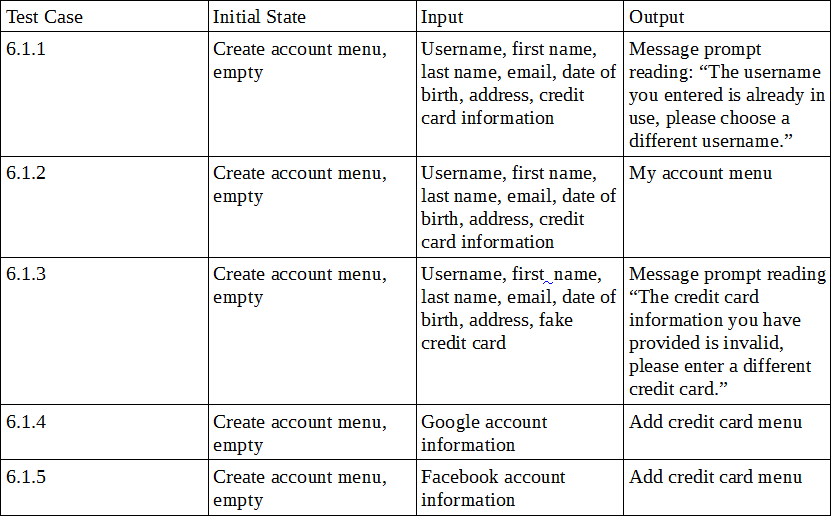
\includegraphics[width=\textwidth,height=\textheight,keepaspectratio]{accountTC.png}


\subsection{Order Transaction}
Smart-Waiter needs to ensure that a user can send in their order, and pay for their order easily and securely. Order transaction will be vigorously tested to ensure complete customer satisfaction.  
\subsubsection{Test Type}
Manual, functional dynamic test 
\subsubsection{Test Factors}
Correctness, reliability, data integrity, data security, ease of use, 
\subsubsection{Inputs}
A set \texorpdfstring{n\textsubscript{i}}{ni} of 10 random orders consisting of different menu items, created manually, where i = 0, 1, 2 .. 9, where i = 0..4 are invalid orders with respect to the restaurant's policies and where i = 5..9 are valid orders. \\
A valid credit card \\
An expired credit card \\
A fake credit card \\
A VISA debit card \\
A VISA gift card \\
\subsubsection{Outputs}
An order summary \texorpdfstring{O\textsubscript{i}}{Oi}, where i corresponds to the \texorpdfstring{i\textsuperscript{th}}{ith} order from the set of orders \texorpdfstring{n\textsubscript{i}}{ni}. \\
A message M, containing either a success or failure message, depending on the card type used. 
\subsubsection{Initial State}
Order Test Cases: Restaurant menu module
Credit Card Test Cases: Payment confirmation menu
\subsubsection{Methods of testing}
Dynamic testing is used to ensure validity, record the number of successful tests given a sample.
\subsubsection{Test Cases}
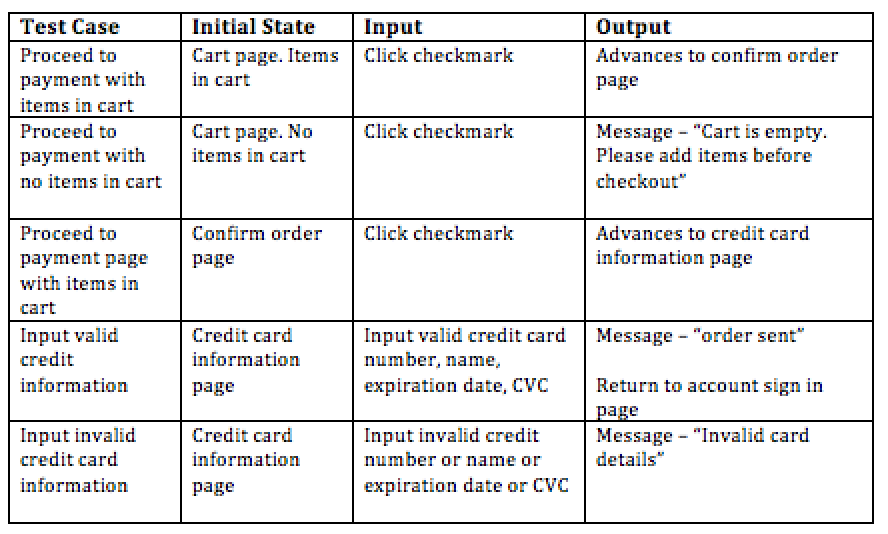
\includegraphics[width=\textwidth,height=\textheight,keepaspectratio]{orderTransactionTC.png}

\subsection{Usability Testing}
\subsubsection{Test Factors}
\subsubsection{Inputs}
\subsubsection{Outputs}
\subsubsection{Initial State}
\subsubsection{Methods of testing}
\subsubsection{Test Cases}

\subsection{Performance Testing}
\subsubsection{Test Factors}
\subsubsection{Inputs}
\subsubsection{Outputs}
\subsubsection{Initial State}
\subsubsection{Methods of testing}
\subsubsection{Test Cases}

\section{Automated Testing Plan}


\end{document}